\scanpage{113}

\mspage{119}
\margin{$\unsure{\times|\ast}$}

\uline{Prop. \deleted{\unsure{6}}7} Soit $f:X\longrightarrow Y$ dans $\mathrm{Diag}$. Conditions équivalentes :

a) $f$ est une $\mathbb D$-équivalence ``universelle'', i.e. pour tout $Y'\longrightarrow Y$ de $\mathrm{Diag}$, $f':X'=X\times_Y Y'\longrightarrow Y'$ est une $\mathbb D$-équivalence.

b) $f$ est une $\mathbb D$-fibration à fibres $\mathbb D$-asphériques.

\uline{Définition 4} Sous les conditions équivalentes de la prop. 6, on dit que $f$ est une $\mathbb D$-fibration \uline{triviale}.

\margin{\figure{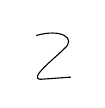
\begin{tikzpicture}[x=0.46cm,y=0.46cm]\draw (0,1.25) .. controls (0.7,1.45) and (1.12,1.17) .. (0.77,0.88) .. controls (0.5,0.61) and (-0.22,0.06) .. (0.12,0.04) -- (0.96,0.1);\end{tikzpicture}}}

Mais attention, $f$ peut-être une $\mathbb D$-fibration et une $\mathbb D$-équivalence, sans que la $\mathbb D$-fibration soit triviale i.e. sans que les fibres soient $\mathbb D$-asphériques, cf p. \unsure{87|85} ff. Et \unsure{ici même|certainement|sûrement} (devrais \unsure{remontrer|remonter}) même si $\mathbb D$ satisfait $\mathrm{Der}\,3\,b_2$ (la plus forte des variantes de $\mathrm{Der}\,3$), donc quand \uline{toutes} les conditions de la prop. 5, y inclus a'), sont équivalentes, celles-ci (i.e. que $f$ soit une $\mathbb D$-fibration) n'impliquent pourtant pas, en général, que dans la condition a') on puisse se borner à $p:Y''\longrightarrow Y'$ une $\mathbb D$-équivalence (au lieu d'une Hot-équivalence) : En d'autres termes, si on a un diagramme cartésien dans $\mathrm{Diag}$

\margin{\figure{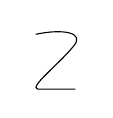
\begin{tikzpicture}[x=0.48cm,y=0.48cm]\draw (0,1.52) .. controls (0.76,1.68) and (1.29,1.55) .. (1.01,1.22) .. controls (0.64,0.75) and (-0.20,0.11) .. (0.05,0.07) -- (1.05,0.07);\end{tikzpicture}}}

\diagram{\begin{tikzcd}[ampersand replacement=\&,row sep=small,column sep=small]
X \arrow[d,"f"'] \& X' \arrow[l,"q"'] \arrow[d,"f'"]\\
Y \& Y' \arrow[l,"p"]
\end{tikzcd}},

avec $f$ une $\mathbb D$-fibration, et $p$ une $\mathbb D$-équivalence, \unsure{il|et} \unsure{ne|on} s'ensuit pas forcément que $q$ soit une $\mathbb D$-équivalence. (Mais ce sera pourtant le cas, \inserted{au moins} si $\mathbb D=\mathrm{HOT}$)

% archive sheet number: 113
